\documentclass{thesis-ekf}
\usepackage[T1]{fontenc}
\PassOptionsToPackage{defaults=hu-min}{magyar.ldf}
\usepackage[magyar]{babel}
\footnotestyle{rule=fourth}
\usepackage{mathtools,amssymb,amsthm,pdfpages,listings,url}
\newtheorem{tetel}{Tétel}[chapter]
\theoremstyle{definition}
\newtheorem{definicio}[tetel]{Definíció}
\newtheorem{megjegyzes}[tetel]{Megjegyzés}
\DeclareMathOperator{\arctg}{arctg}
\renewcommand{\lstlistingname}{Programkód}
\lstset{
	inputencoding=utf8/latin2,
	language=C++,
	basicstyle=\footnotesize,
	numbers=left,
	breaklines,
	postbreak=\hbox{$\color{red}\hookrightarrow\ $},
	xleftmargin=1cm,
	xrightmargin=1cm,
	backgroundcolor=\color{gray!10},
	frame=tlbr,
	framesep=3pt,
	keywordstyle=\bfseries\color{blue},
	stringstyle=\bfseries\color{red},
	commentstyle=\bfseries\color{green},
	morecomment=[l][\color{magenta}]{\#},
	showstringspaces=false
}

\begin{document}
\institute{Matematikai és Informatikai Intézet}
\title{Programozható elektronikák alkalmazásai}
\author{Bagoly Gábor\\programtervező informatikus}
\supervisor{Dr. Geda Gábor\\egyetemi docens}
\city{Eger}
\date{2022}
\maketitle
\tableofcontents

\chapter{Bevezetés}\label{ArduinoChapter}

A választott szakdolgozati témám a \emph{Programozható elektronikák alkalmazásai}, azon belül a témám egy okos otthon tervezése, különböző okos eszközök irányításával egy lokális szerveren úgy, hogy azt egy \emph{Raspberry Pi}, vagy \emph{NodeMCU} szolgáltatna, és irányítaná az eszközöket.
Az eszközökkel például világítást, fűtést is lehet vezérelni, akár automatikusan. Az eszközök különböző féle programozható elektronikák segítségével lesznek megvalósítva. Célom az lenne ezzel, hogy belelássak az okos otthonok működésébe, különböző programozható eszközök alkalmazását jobban megismerjem, és, hogy egy olyan általános kezelőfelületet tudjak létrehozni, amit könnyen tud a felhasználó alkalmazni. Az okos otthon részről pedig majd \aref{smarthomeChapter}.~fejezetnek \pageref{smarthomeChapter}.~oldalától lehet majd többet megtudni, ahol megmutatom azt is, hogy C++ programozási nyelvet használva hogyan olvasom be és, írom ki egy hőmérséklet és páratartalom szenzor által mért adatokat.

\section{Az Arduino platform}
	Az Arduino egy széleskörűen elterjedt, nyílt forrású fejlesztőplatform. Az Arduino-t oktatási céllal hozták létre, de előszeretettel használják otthoni projektekhez, a kisebb automatizálási feladatoktól kezdve az okos otthonok kialakításáig. Ezek mellett ma már az ipari alkalmazások sem ritkák és rengeteg IOT eszköznek is az alapja.
	Az Arduino platform része egy elektronikai áramköri lap és a szoftveres környezet. Maga az áramköri lap nagyon sokféle felépítésben megtalálható.

\section{Arduino UNO felépítése és tulajdonságai}\label{arduinoUnoSection}
Az egyik legelső és leginkább elterjedt áramkör az Arduino UNO.

\begin{figure}[ht!]
	\centering
	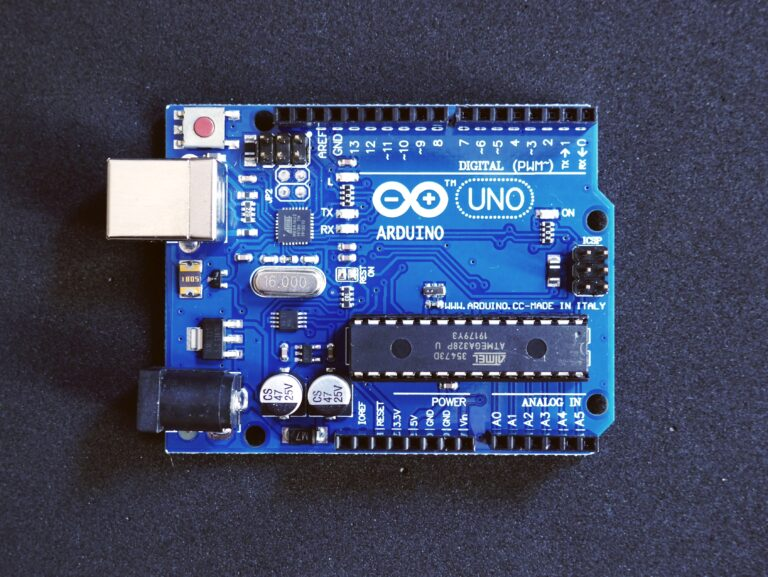
\includegraphics[width=5cm]{arduinoUno.jpg}
	\caption{Az \emph{Arduino UNO} áramköri lap az egyik legelterjedtebb a sokféle kártya közül.}
	\label{fig-arduinoUno}
\end{figure}

Az Arduino áramkörök leglényegesebb alkatrésze a mikrovezérlő. Az \emph{UNO} esetében ez egy \emph{ATmega328/P} típusú, 8 bites mikrovezérlő. A mikrovezérlő egy integrált áramkör (IC, chip), amiben a processzor és a memória mellett számos egyéb periféria is megtalálható. A legfontosabb perifériák egy általános mikrovezérlőben a következők lehetnek: időzítő áramkörök, analóg és digitális be- és kimenetek, kommunikációs perifériák és még sok egyéb. Ilyen mikrovezérlőkből egyre több található meg a minket körülvevő hétköznapi használati tárgyainkban is, háztartási kis- és nagy gépekben például: mosógépben, digitális órában, távirányítóban, mobiltelefonban. Segítségükkel mérhetjük szenzorok jelét, beolvashatjuk nyomógombok állapotát, vezérelhetünk velük LED-eket, motorokat, kommunikálhatunk más áramkörökkel és még sok egyéb feladatra használhatók.

Az \emph{Arduino UNO} áramköri lap szerepe, hogy a rajta elhelyezett mikrovezérlőnek a lábai ki vannak vezetve egy kényelmesen hozzáférhető és könnyen használható csatlakozókra, valamint megtalálható rajta a mikrovezérlő működéséhez és programozásához szükséges egyéb alkatrészek.

A mikrovezérlők általában lényegesen kisebb számítási teljesítménnyel rendelkeznek egy hagyományos PC-hez képest, de ezáltal sokkal alacsonyabb a fogyasztásuk és méretük is jelentősen kisebb lehet. Mivel általában nem fut rajtuk operációs rendszer, ezért a rendelkezésre álló erőforrásnak megfelelő valós-idejű feladatokra is alkalmazhatók, azaz egy adott eseményre a mikrovezérlő gyorsan és egy garantált maximális idő alatt képes reagálni.\footnote{Léteznek valós idejű operációs rendszerek, azonban ezek több erőforrást is igényelnek, mint a natív kód.}  Az \emph{ATmega328/P} típusú mikrovezérlő lényegesebb paraméterei:

\begin{itemize}
	\item 8\,bites architektúra
	\item 16\,MHz-es órajel
	\item EEPROM (csak olvasható memória): 1\,KB
	\item SRAM (változók tárolására): 2~KB
	\item A flash (programot tároló ROM): 32\,KB
\end{itemize}

\begin{figure}[ht!]
	\centering
	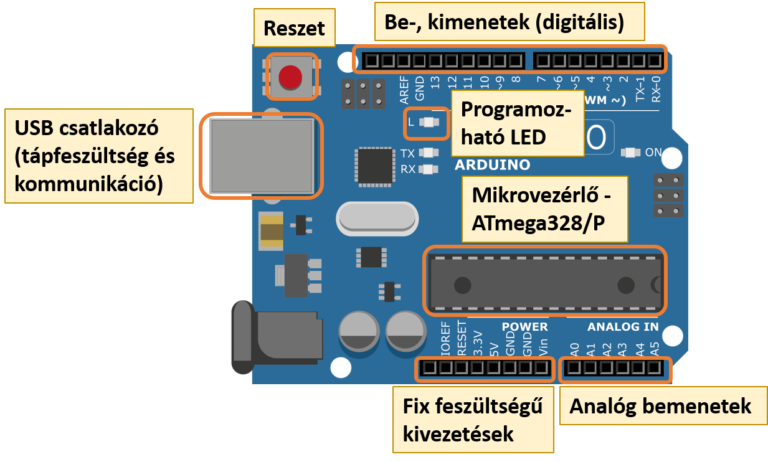
\includegraphics[width=8cm]{arduinoUnoFelepites.png}
	\caption{Az \emph{Arduino UNO} áramköri lapon lévő legfontosabb alkatrészek}
	\label{fig-arduinoUnoFelepites}
\end{figure}

Ahhoz, hogy külső áramköröket is használjunk, tudnunk kell a lábkiosztást, azaz, hogy a kódból hogyan tudunk hivatkozni az adott kivezetésre. A Arduino áramköri lap két szélén lévő tüskesor aljzat melletti számokkal érjük el az adott kivezetést a kódból. Ezek a kivezetések lehetnek digitálisak (0-tól 13-ig jelölve) vagy analóg bemenetek (A0-tól A5-ig jelölve). Az A0-A5 kivezetések még digitális be- és kimenetek is lehetnek, ha a kódban úgy állítjuk be az adott kivezetést. Külső áramkörök esetén a fix feszültségű kivezetésekről kényelmesen tudunk tápfeszültséget adni az áramkör számára.

A csatlakozókhoz kényelmesen köthetünk szenzorokat, digitális IC-ket és egyéb külső áramköröket. Ahhoz, hogy ezeket biztonságosan tudjuk használni, előbb meg kell ismernünk a be- és kimenetek működésének korlátait. A témához szükséges ismerni a következő, legfontosabb szinteket és korlátokat:

\begin{itemize}
\item Működési feszültség: 5\,V
\item Maximális kivehető/befolyatható áram egy digitális kimenetből: 20\,mA
\item Maximális kivehető áram a 3,3\,V-os kimenetből: 50\,mA
\end{itemize}

Az feszültségszintekre és áramkorlátokra nagyon figyelni kell az Arduino használata során. Csak egyforma feszültségszinteken üzemelő áramköröket szabad összekapcsolni, az áramerősségeket pedig a számolás során kapott értéknek megfelelő, sorba kapcsolt ellenállással lehet a maximális megengedett érték alatt tartani.

Az Arduino-hoz számos ,,feltét'' áramkör is kapható, amiket Arduino shield-eknek neveznek. Ezeknek az áramköri lapoknak az az előnye, hogy egyszerűen, egyetlen mozdulattal rá lehet helyezni az Arduino-ra és máris kiegészítettük az Arduino-t valamilyen hasznos funkcióval. A kompatibilitásra figyelni kell, mert léteznek 3,3\,V tápfeszültséget igénylő shieldek, amik tönkremehetnek az 5~V-os jelszintet használó \emph{Arduino UNO}-tól.
További Arduino eszközről az alábbi könyvben tudhat meg többet.\cite[8--12.oldal]{arduinoBook}

\chapter{IoT eszközök alkalmazása okos otthonban}\label{smarthomeChapter}
\section{IoT eszközök}
Manapság számos kis és nagy háztartási készülék és gép érhető el okos kivitelben. Ezek úgynevezett IoT (Internet of Things) eszközök, amelyek az otthoni WiFi hálózaton keresztül egyszerűen párosíthatóak az adott gyártói applikációval. Erre azért van szükség, hogy a lehető legtöbb okos funkciót ki tudjuk használni, illetve esetleges firmware frissítéseket el tudjunk végezni. Ezzel a módszerrel azonban szinte minden márkához és eszközhöz külön applikációt kell használni, ezáltal egyfajta szigetüzem jön létre.

Manapság már beszerezhető például okos WiFi-s mosógép, ahol külön alkalmazáson keresztül nyomon követhetjük, mikor jár le a mosás. De automatizációval előre meghatározott időpontban is elindíthatjuk a mosógépet. Ha nem vagyunk otthon a vízérzékelők figyelik, hogy nincs-e probléma, és szükség esetén gondoskodnak a víz elzárásáról.

IoT eszközök beszerzésével tehát elérjük, hogy a különböző gépek wifin vagy más protokollokon keresztül képesek egymással kommunikálni. De ha nem időben gondolkodunk rendszerben, akkor könnyen eljuthatunk oda, hogy minden gyártóhoz egy külön alkalmazást rendelünk, ami egyre bonyolultabbá teszi az egyes eszközök kezelhetőségét és ellehetetleníti az automatizációt. IoT eszközök közé tartozik \aref{arduinoUnoSection}.~szakaszban említett \emph{Arduino UNO} is.

Ellentétben a ,,kész'' rendszerekkel vagy DIY\footnote{Do It Yourself, azaz magyarul Csináld Magad módszer.} megoldásokkal az egész háztartást összeköthetjük egy rendszer égisze alatt. Az okos otthon megalkotása során elindulhatunk nagy gyártók\footnote{Az alábbiak például: Chameleon Smart Home, Zipato vagy Loxone.} szisztémái mentén, de nyílt forráskódú rendszerek mellett is dönthetünk.

Az otthonok automatizálására egyszerű “barkácskörülmények” között is lehetőség van, így egyre többen használnak Raspberry Pi-t például FHEM, Domoticz vagy Node~RED szoftverrel, amihez külön szerzik be az egyes érzékelőket, reléket és a különböző bővítő modulokat, a kontrollálni kívánt eszközöket, a vezérlő szoftvert, illetve a helyi vagy távoli vezérlőegységet. A beszerzés után ezeket manuálisan kell egy rendszerbe kötni és beprogramozni az automatizációkat. 

Az IoT eszközök a felhasználási terület alapján az módon kategorizálhatóak:
\begin{itemize}
	\item Industrial Internet Of Things\footnote{Magyarul: Ipari Dolgok Internetje.}
	\begin{itemize}
		\item Az eszközök alkalmazása ipari, szállítási, energetikai, vagy egészségügyi területen.
		\item Az adatok mennyisége és sebessége a tartóstól a viszonylag magasig terjed.
		\item Az alkalmazások biztonság-kritikusak, például egy intelligens közlekedési rendszer hibás működése veszélyeztetheti az emberek életét.
		\item Az IIoT alkalmazások rendszerközpontúak.
	\end{itemize}

	\item  Consumer Internet Of Things\footnote{Magyarul: Fogyasztói Dolgok Internetje.}  
	\begin{itemize}
		\item Fogyasztói eszközök, például mobil, hűtőszekrény, szemüveg stb.
		\item Az adatok mennyisége és sebessége viszonylag alacsony.
		\item Az alkalmazások nem túl kritikusak, például a fitnesz modulok meghibásodása nem okoz kárt.
		\item A CIoT alkalmazások fogyasztóközpontúak.
		\item CIoT még ezen belül az alábbi kategóriákra bontható:
		\begin{itemize}
			\item Személyes IoT.
			\item Csoportos IoT
			\item Közösségi IoT
		\end{itemize}
\end{itemize}
\end{itemize}

 \lstinputlisting[caption=Hőmérséklet és páratartalom szenzor által mért értékek mérése és kiírása]{cppCode.cpp}

\section{Okos otthon}
Egy tudományos cikk alapján az okos otthon az alábbi módon definiálható:
\begin{definicio}\label{smarthomeDef}
,,az okos otthon egy olyan (a lakhelyünkön kiépített) platform, ami IoT-s, kommunikációs  és különböző számítógépes technológiákat felhasználva eszközöket köt össze egymással egy hálózaton keresztül úgy, hogy ezek automatizálhatóvá és könnyebben irányíthatóvá és váljanak, ezzel javítva az egész rendszer (ház) kezelhetőségét, kényelmét és biztonságát.''\cite{smarthome}
\end{definicio}
Sok ember megpróbált részletesebb kritériumot is adni az okos otthonokra. \textsc{Michael C. Mozer} szerint egy épület csak akkor tekinthető intelligensnek, ha képes irányítani a világítást,
a fűtést, hűtést és a redőnyöket \footnote{Továbbiakban olvashat erről \textsc{Michael C. Mozer}: Lessons from an Adaptive Home című írásában.\cite{Mozer}}, habár ez a megközelítés pontatlan. Szerintem nem kell ennyire szigorúan megszabni, a ház mely részeit kell irányítania egy ilyen rendszernek, csak arra kell törekednie, hogy a felhasználó életét megkönnyítse és
segítse anélkül, hogy zavaróvá válna.

\subsection{Okos otthon kiépítése}
Az okosotthon\footnote{Melyet \aref{smarthomeDef} definíció kifejt.} kiépítése során az első és legfontosabb kérdés, hogy a különböző protokollon kommunikáló eszközöket hogyan fogjuk össze és vezéreljük. Ehhez meg kell vizsgálni, hogy az okoseszközök milyen kompatibilitással rendelkeznek.

A nyílt forráskódú, otthonautomatizálási platform, az OpenHab segítségével számos eszközt és rendszert integrálhatunk. Ezáltal létrejön az egységes felhasználói felület, viszont mindez időigényes folyamat, amely komoly precizitást és hozzáértést igényel. A lépéseket akár az interneten keresztül is nyomon követhetjük, YouTube videók által is megtanulható, konfigurálható.

A Home Assistant open-source\footnote{Magyarul: nyílt forrású.} szoftver szintén népszerű Magyarországon, ami a vezérlés mellett az adatvédelmet is előtérbe helyezi. Sok angol és több magyar nyelvű fórumon tájékozódhatunk, kérdezhetünk másoktól, amire általában szükség is van, mert könnyű elakadni a beállítási lehetőségek rengetegében.

Az okosotthon házilag való telepítése ugyanakkor kockázatokkal is jár. Amennyiben problémák lépnek fel, megfelelő szaktudás nélkül nehezebb helyrehozni azokat, például szoftverfrissítések esetén vagy az eszközök meghibásodásánál. Gondoljunk csak bele, hogy egy rendszerhibánál működésképtelenné válik az otthonunk. Ha csak a világításvezérlés nem működik a probléma orvoslásáig, talán nem okoz életbevágó problémát, de a fűtésvezérlés egy hideg téli estén már annál inkább.


\chapter*{Összegzés}
 \Az{\eqref{matKeplet}} képleten pedig látható az, hogy a \LaTeX~mennyire alkalmas matematikai  képletek megjelenítésére.
 
\begin{equation}\label{matKeplet}
	g\colon \mathbb{R} \setminus \left\{\frac{k\pi}{2}:k\in \mathbb{Z}\right\}\rightarrow \mathbb{R},\quad g(x)\coloneq
	\begin{cases}
		\frac{\arctg^2(x+\pi)}{\sin(2x)},&\text{ha }x\geq\frac{2}{3},\\
		\cos^4(5x), &\text{különben.}
	\end{cases}
\end{equation}



\begin{thebibliography}{2}
\addcontentsline{toc}{chapter}{\bibname}
\bibitem{arduinoBook}
\textsc{Jeremy Blum}: \emph{ Exploring Arduino: Tools and Techniques for Engineering Wizardry}, 2019.
\bibitem{smarthome}
\textsc{Smart Home:}\emph{ Architecture, Technologies and Systems}

\url{https://tinyurl.com/smarthomeBook}
\bibitem{Mozer}
\textsc{Michael C. Mozer:} \emph{Lessons from an Adaptive Home, University of Colorado}

\url{ https://tinyurl.com/MozerBook}
\end{thebibliography}

\end{document}